% This example An LaTeX document showing how to use the l3proj class to
% write your report. Use pdflatex and bibtex to process the file, creating 
% a PDF file as output (there is no need to use dvips when using pdflatex).

% Modified 

\documentclass{l4proj}
\usepackage{url}
\usepackage{color}
\usepackage{graphics,graphicx}
\usepackage{epsfig}
\usepackage{epstopdf}
\usepackage{colortbl}
\usepackage{multirow}
\usepackage{booktabs}
\usepackage{ifthen}
\usepackage{float}
\usepackage[biblabel]{cite}
\usepackage[numbers]{natbib}
\usepackage[breaklinks,colorlinks,citecolor=black,urlcolor=black,linkcolor=black,pdfpagelabels=false]{hyperref}
\usepackage{mathtools}
\usepackage{wrapfig}
\usepackage{caption}
\usepackage{subcaption}
\usepackage{enumitem}
\usepackage{amssymb}
\usepackage{array}
\usepackage{threeparttable}

\begin{document}

\newcommand{\todo}[1]{\textcolor{red}{#1}}
	
	
\title{Walk Around The World}
\author{Ryan Wells - 1002253w}
\date{\today}
\maketitle
\begin{abstract}

This project aims to encourage users to do outdoor cardiovascular
exercise by gamifying the experience with positive encouragement
through a mobile application. By tracking the distance the user
travels in each exercise session through device GPS and translating
this into well-known outdoor pursuits allows the user to quantify
their exercise in terms of well known physical and cultural
achievements. These achievements will take badge-like form where an
incremental reward structure will be used to encourage the user. 

%% Outdoor pursuits will contain: actual routes such as the West Highland
%% Way and the climb to the top of Everest; popular culture references
%% such as ``Route 66'' and the (approximate) distance that \emph{Frodo}
%% and \emph{Sam} travelled in J.R.R.Tolkein's ``The Lord of the Rings'';
%% and Global distances such as the distance between capitol cities and
%% simple metrics such as the first one hundred miles. 

%% The user will exercise with a compatible device on their
%% person. During exercise the device will track and log the distance
%% that the user has travelled and add this to their accumulators. If
%% this device is their smart phone then the Mobile Application will
%% notify them immediately when they have completed an outdoor pursuit,
%% otherwise they will be notified when data is collected from the
%% dedicated hardware.

%% This application will encourage social exercise through outdoor
%% pursuits that can only be completed through teamwork with other users
%% that have met in real life. This intends to extend the influence of
%% rewarding exercise by encouraging users to include their peer group in
%% exercising with them and sharing their successes. For a user,
%% this is incentivised by unlocking achievements only achievable through
%% this social interaction.

An analysis of frequency and duration of exercise with regards to
duration of application use will be used with user feedback to
indicate whether or not gamification techniques could have a valid
application in cardiovascular exercise.  

\end{abstract}
\educationalconsent
\tableofcontents
%==============================================================================
\pagebreak
\pagenumbering{arabic}
\chapter{Introduction}\label{ch_intro}

\section{Motivation / Context}
The number of smartphones being sold per year is
increasing\cite{phones_gartner, phones_guardian} and nearly
three-quarters of exercisers use technology to support their
workouts in some way\cite{lifefitness}. This project aims to utilise
this mass market 
acceptance of technology in exercise and combine it with game like
elements to evaluate the effects of games and
exercise. Specifically, this project will look at outdoor
cardiovascular exercise where the user is required to exercise with
their phone with them.Studies have shown that physical exercise
between 1 hour a day for children over five years of age and as
little as 2.5 hours a week for adults has a huge positive impact on
our physical and emotional wellbeing\cite{govsurvey, amsurvey} .

The 2006 Health Survey for England\cite{exercise} states that: 
\begin{quote}
  Physical inactivity is associated with all-cause mortality and
  many chronic diseases, including ischaemic heart disease, diabetes,
  certain cancers, and obesity \dots \ Many people attribute their
  failure to achieve the target recommendations to a lack of time to
  take exercise. 
\end{quote} 
We intend to approach this problem by targeting the perception that
there is a ``lack of time to take exercise''. 

A later Health Survey for England in 2012 noted that the change in
definition as to what the exercise guidelines were implied that more
people than before were meeting the exercise guidelines
\cite{exercise_2012}. These guidelines allow for exercise sessions of
10 minutes or more where previously exercise only counted if it was
more than 30 minutes in length. Automatically this will include
more people than the previous survey as the criteria is less
restrictive, however we can use this to our advantage..

Since the guidelines now allow exercise sessions that can be as little
as 10 minutes we can use this to deal with the ``lack of time to take
exercise'' excuse and encourage users to use these small time
intervals to undertake exercise. 

\section{Problem Statement}

The application of game like elements to exercise is nothing new. As
will be discussed in Section \ref{sec_comparison}, other applications
have taken different approaches to incentivising exercise. To the best
of my knowledge no other product uses exactly the same experience
as the one proposed in this dissertation.

The aim of this project is to create a gamified experience for outdoor
exercise, specifically walking, jogging and running. By creating a
gamified experience we aim to encourage and incentivise users to
exercise. 

\section{Targeted users}
\label{sec:targeted_users}
Consider an individual who has a relatively short distance to travel,
such as a commute to work,
and who doesn't exercise regularly. This individual could either
travel this distance on their own accord or use a service such as a
car or take public transport. With no external encouragement, and low
self control, the individual may be likely to take the car or public
transport and lose out on all benefits of exercise. 

By gamifying this travel time we hope that the user decides not to
take public transport or travel by car so that they can achieve the
goals of the game. This positive encouragement will help the user to
begin exercising and be rewarded for doing so. Gradually over time as
users start to engage with the game more often we hope that users
start to willingly extend their commute, colloquially ``taking the
long route'', or simply exercise more often just to ensure that they
receive an achievement. If this happens then the game has been
successful as through using this application the user has exercised
more than they would have without it. The short term rewards will
initially help these users the most: since they do not exercise
often they may need quicker encouragement to help push them to
exercise more regularly.

Also consider a user who frequently exercises and repeatedly travels
the same route, or the same collection of routes when exercising. This
individual may easily tire of the journey or bad weather may
discourage the individual just enough that they decide to move their
exercise to a controlled environment such as a gym where the benefits
are not as profound, or give up entirely. 

If we can encourage this user to continue exercising by giving the
user a reward structure they wish to invest in then we can help this
user continue to benefit from exercise. In this case the game is a
success if it diverts the user from changing away from their current
exercise regime. Long term rewards will benefit these users as they
can use these to help encourage themselves to maintain the current
rate that they are exercising at. These will be reinforced with the
rewards from the short term goals in a similar way to the previous
example. 

\section{Summary of Contributions}

This report presents the following contributions: 

\begin{itemize}
  \item A brief overview of gamification;
  \item An analysis of the current state of the market for exercise
    apps and devices;
  \item An exploration of the requirements, design decisions and
    implementation of ``Urban Explorer'' - the application built for
    the analysis of this type of gamification;
  \item The ``Urban Explorer'' application, which can also be found on
    the Google Play Store \cite{app_store_link};
  \item The results from user evaluation and testing.
\end{itemize}

\section{Outline of the Report}

We will start by examining the current state of the market in Chapter
\ref{ch_background} by
discussing other implementations of gamification in mobile
apps. Through this examination, we will discover the benefits and
pitfalls of each implementation and use this to form the basis of our
implementation. 

We define the overall goals of the project in Chapter \ref{ch_method},
specifically how we will use gamification to deliver our
implementation and what we hope to achieve in the scope of this
project.

An analysis of our implementation will then be presented in Chapter
\ref{ch_results}. This is based on user testing and experience, and evaluation of the
overall suitability of the platform.

\chapter{Related Work and Background}\label{ch_background}

\emph{Life Fitness} in 2012 released a survey concerning technology in the
exercise environment\cite{lifefitness} where it was found that over
half of gym users used a smart phone or tablet when exercising. This
study focused solely on gym users which is not our target market for
this product (we are targeting users who exercise outdoors), however
it is not unreasonable to assume similar statistics for our target
demographic. We use this metric along with the vast user base of the
related applications we compare in Section \ref{sec_comparison} as a
basis of platform validity. 

\section{Gamification}
\citet{gamification_book} define gamification as ``The process of
game-thinking and game mechanics to engage users and solve
problems.''. There are four main building blocks to this definition:

\begin{description}[style=multiline, leftmargin=3cm]
\item[\emph{game-thinking}] What the users thoughts should be when
  they are interacting with this game and how the user should perceive
  their interaction.
\item[\emph{game mechanics}] How we provide this game-like
  experience. What metrics we use to indicate success and encourage
  play. 
\item[\emph{users}] What user group this gamification is intended for
  and who we hope to influence the most through this application.
\item[\emph{problems}] What issues are we trying to fix or improve
  through this application of gamification.
\end{description}

\citet{artOfGameDesign} proposes four main elements, the ``elemental
tetrad'', that form a game: \emph{mechanics}, \emph{story},
\emph{aesthetics}, and \emph{technology}. These four elements influence
how a user perceives a game (\emph{game-thinking}) and
\citeauthor{artOfGameDesign} proposes that all four should be treated with
equal weighting to achieve a successful game. An engrossing
\emph{story} combined with good \emph{aesthetics} can be used to mask
what a user is truly doing. Recently, \citet{genesInSpace}
released a game called \emph{Genes In Space} where users chart a
course through space to pick up as much ``Element Alpha'' as they can
while destroying asteroids. The route they chart is based on a space
map where the distribution of ``Element Alpha'' is shown and
collecting ``Element Alpha'' allows the user to buy upgrades to their
spaceship to personalise and improve it. The distribution of ``Element
Alpha'' is based on a sample of a DNA microarray from a cancer patient. The 
course you plot identifies where alterations in the genome have
occurred. By applying game elements the user plots a course that will
maximise their success (\emph{game mechanic}) while they are also
identifying key areas of interest that will benefit cancer
researchers. 

A similar application for protein folding is utilised by the \emph{Foldit}
project by \citet{foldit}. Here users are challenged directly to
manipulate a protein chain to find an optimal layout of this chain (a
fold) based on a set of given criteria. This solution allows
suggestions to be proposed by the community and reviewed by scientists
to determine their merit. There is a points based \emph{game mechanic}
where optimal layouts are rewarded with more points than less optimal
solutions. A benefit to this application of gamification is that it
saves a substantial amount of the scientists time. The scientist only
has to review the submitted protein fold instead of designing it,
which is a significantly shorter time investment.

In both of the applications of gamification above the \emph{problems}
have been of a scientific nature and the \emph{users} have been casual
gamers, scientists and researchers. Gamification has been shown to
bring improvements in domains other than medical research.

\emph{World Without
  Oil}\footnote{\url{http://www.worldwithoutoil.org}} was an Alternate
Reality Game created to explore the ways to conserve oil resources
during a shortage where 1,700 players were involved in the project
over a 32 day period. \citet{reality_broken}, one of the designers
involved with \emph{World Without Oil}, commented about the
behavioural change benefits of games:

\begin{quote}
  We can change our real-life
  behaviours in the context of a fictional game precisely because there
  isn't any negative pressure surrounding the decision to change. We
  are motivated purely by positive stress and by our own desire to
  engage with a game in more satisfying, successful, social and
  meaningful ways.
\end{quote}

The \emph{problems} here were based on a contrived situation, but
\citeauthor{reality_broken} notes that when there was a gas crisis a
year later players of \emph{World Without Oil} were in a significantly
better situation than those who were not. This application of
gamification allowed these users to positively benefit in a real world
situation that was similar to one experienced in game.

A final example closer to the problem domain of this project is
\emph{Chick Clique} (\citet{chick}) which uses social game elements to
encourage a peer group of four teenage schoolgirls to exercise. Each
student was given a personal digital assistant (PDA) and a pedometer
to track the steps they take. The steps taken can be compared with the
other three peers in their group to gauge personal progress. Help was
also provided where the user could get information about fast-food in
terms of how many steps were required to ``walk off'' the empty
calories. Although this was a small experiment it was met with good
feedback from the test group who commented that breaching the subject
of healthy eating and exercise within the group was as valuable as the
tracking and suggestion the product gave. This is another example
where gamification has positive side effects outside the game
environment.

\section{Comparison of related applications}\label{sec_comparison}
Incentivising exercise is not a new concept in the mobile market. From
simple applications that mimic a pedometer to immersive alternate
realities, there has been a varied approach to encouraging
exercise. These approaches can be shown through the following
applications. 

Table \ref{table:competitor_comparison} gives a brief
overview of requirements and user statistics for the compared products
gained from the Google Play Store.

\begin{table}[h]
  \centering
  \begin{tabular}{ | c | c | c | c |} \hline
    Name & Interface & Requirements & User base  \\ \hline
    Charity Miles & Mobile App & App and GPS & 10K - 50K\cite{charitymiles_store}\\ \hline
    Zombies, Run! & Mobile App & App and GPS, headphones & 100K - 500K\cite{zombiesrun_store}\\ \hline
    WalkJogRun & Mobile App & App and GPS  & unknown \\ \hline
    Fitbit & Dedicated hardware and Mobile App & Dedicated Hardware & 1M - 5M\cite{fitbit_store}\\ \hline
  \end{tabular}
  \caption{Comparison of exercise gamification implementations from
    the Google Play store}
  \label{table:competitor_comparison}
\end{table}

\subsection{Charity Miles}
\label{sec:charity_miles}
\emph{Charity Miles} encourages you to exercise by facilitating you to raise
awareness of charities and help
others as you exercise. For every mile that you run or walk \$0.25 is
donated to a charity of your choice, and for every mile you cycle \$0.10
is donated. The money currently comes from a pool of \$1,000,000
gathered by the parent company so you as an end user don't have to pay
anything. 

The money you accrue during an exercise session is called your
``sponsorship'' and is only passed onto your charity when you share
your success to a social network (Facebook or
Twitter)\cite{charitymiles_terms}. \emph{Charity Miles} say this is to
increase awareness of the charity, but it is also a good advertising
tool for them.

The incentive here is clear - run to donate. In essence, you are both
being paid to exercise and you are exercising to help out a
charity. The monetary backing allows you to quantify your exercise in
terms you are very familiar with whilst generating a feeling of
satisfaction by helping a charity.

The main drawback here is that there is no defined behaviour for what
happens when the \$1,000,000 pool runs out. From a business
perspective, the app could easily be re-purposed for non-centralised
pool funding where the end user could find local sponsorship. However
this entirely changes the user experience and explicitly requires
effort on the users side to gather this sponsorship. 

\subsection{Zombies, Run!}
\label{sec:zombies}
\emph{Zombies, Run!} is a companion app that encourages you to exercise through
audio cues, rich story and a base-building game. As you run you are
being ``chased'' by a hoard of zombies that get closer and further
away from you as you exercise. This is indicated through audio cues-
the closer they are to catching you the louder they become. 

The app creates an alternate world where you are defending your
stronghold from a zombie invasion and you are required to leave the
base to gather supplies. The story narrative tells you what you need
to gather and you find these supplies based on the distance you travel
and the route you take. Your success is measured by the fortifications
and of your base, which you can improve and personalise by running
faster/further than you have done before. 

You are required to wear headphones and carry your mobile phone while
exercising. The headphones give you audio queues to immerse you in the
story, but it is a requirement of the game experience that you listen
to the soundscape provided. As endearing as groaning zombies may be,
it is understandable that users may tire of hearing it. Also, a user
may be used to listening to their own music and use that to zone out
of the exercise, so the interruption by the undead may make some users
reluctant to adopt this.


\subsection{WalkJogRun}
\label{sec:walkjogrun}
\emph{WalkJogRun} helps you discover new routes that are geographically
close to where you are and record your favourite routes to share with
your friends. From your current location it finds and
proposes new exercise routes given a certain route length. It can
provide turn-by-turn direction help when you are exercising to ensure
you do not get lost and will also record an exact route as you run so
you can create a new route with the minimum of effort. 

Your workout is saved and can be later analysed so you can accurately
monitor your progress. You can also share this workout within your
peer group which brings social interaction into the exercise domain.

Since the routes are user provided, there is no guarantee that the
routes are safely traversable or applicable to all types of exercise -
a route that can be walked may not be applicable for a runner due to
terrain type, for example. 

There is no clear gamified experience in this application, so the
incentive is self-provided. The user can only use this to improve
their exercise experience as there is not much in the way of
encouragement. It is included in this comparison as although it is not
gamified it still has the potential to encourage users.

\subsection{Fitbit}
\label{sec:fitbit}
I have included a comparison with \emph{Fitbit} products to display other
mediums in which this application can be used. Although it is not
mainly based around a mobile phone use it is an interesting comparison.

\emph{Fitbit} provide a collection of dedicated hardware devices capable of
accurately measuring your distance travelled (and in some models the
height you have ascended in terms of ``flights of stairs'') as a means
of tracking your activity. At the core, it is a glorified pedometer
with web and phone apps to accompany it and display progress. The
devices and apps also make a prediction about the calories you burn each
day based upon the distance you travel when wearing the device, your
weight and stride length. 

Each device can show you the progress toward your daily goal (either
steps taken or predicted calorie burn) with various visualisation
techniques, the simplest of which is a row of five LED lights that
fill up as you near your goal. Synchronisation with compatible phones,
or through a computer if your device is not compatible, allows a more
in depth visualisation of your progress.

The gamification aspect is inherent in the design of these products:
you set your own goal and you can easily view your progress at a
glance. Upon completion of your goal the device vibrates and lights up
to notify you. You are also awarded badges for daily completion such
as walking 10,000 steps a day and lifetime completion goals such as
travelling 100 miles in total.

There is a clear downside to this as you are required to purchase a
bespoke device to fully utilise the experience provided by
\emph{Fitbit}. When compared to an app that may be \$1.99 or thereabouts it is
a much larger start up cost than the previous examples. However this
larger start up cost may be an encouragement itself: the user may
feel obligated to commit to using the device since they are more
financially invested, which may help with the on boarding required to
fully benefit from these systems.

Most of these devices are reasonably discrete, the more advanced the
devices get the larger they become. Since these devices must be worn
mainly on the wrist there are social implications involved. When
creating a product like this we must to consider whether the user
is willing to let everyone know that they are using a fitness tracker.
The other applications are more discreet by design, since they are a
mobile app they can be hidden easier, and so it is less obvious that
you are using a fitness tracker. How subtle and stylish a fitness
tracker is could impact a users willingness to use it in public, which
will affect the overall effectiveness of the product.

\section{Consideration of competitors concepts in this project
  implementation}
\label{sec:consideration}
Each of the above products utilise gamification in an effective way
and each implementation differs in how they utilise game
elements. This project builds upon some of the design decisions these
competitors have used, aiming to remove some of issues that make the
competitors products either unsustainable or flawed.

First and foremost, this project should not require any form of
additional hardware for the end user or monetary investment. A key
demographic that we are targeting are those users who do not exercise
outside often, so we do not want to create a barrier between those
users and them achieving their exercise goal. This is in reference to
the \emph{Fitbit} product discussed in Section \ref{sec:fitbit} which
requires a dedicated hardware wristband, and the \emph{Zombies, Run!}
(Section \ref{sec:zombies}) and \emph{WalkJogRun} (Section
\ref{sec:walkjogrun}) products, both of which require the user to
purchase a mobile app. A monetary investment could be a reason for an
under encouraged user to not take the first step to starting the
exercise process. 

This project should also not require a social aspect to achieve the
core goals for this application, unlike \emph{WalkJogRun} (Section
\ref{sec:walkjogrun}) which has a heavy reliance on social
contributions from users in your area. Although \emph{WalkJogRun} does not
provide a gamified experience, it does enhance your exercise
experience by showing you new running routes. The routes that are
shown as suggestions are entered into the system by other users as
they run. An analysis of crowdsourcing gamified content for exercise
encouragement is outwith the scope of this project due to the number
of players and the length of time required to complete a worthwhile
analysis. It would be interesting future work in the context of this
application, however. 

\emph{Charity Miles} (Section \ref{sec:charity_miles}) also has a social
restriction where the user is required to share to a social networking
site information about the exercise session they have completed before
their charity of choice can receive the money the user has raised. It
can be argued either way as to whether or not this will be an extra
encouragement to the user, but this extra step is an obstacle
between the user and their complete success metric. This project
should endeavour to remove these obstacles that are not related to
their own personal ability: that is to say the user should only be
restricted access to their success metric because of the users effort
did not merit access (a user was not awarded a gold medal because the
user did not deserve a gold medal, not because they did not share
their running time to Facebook).

There should be no limitation to the app because of a reliance on an
outside party. In \emph{Charity Miles} there is a central reserve of
money which you can allocate to your charity of choice by exercising
but there is no defined behaviour for when this money runs out. This
central reserve of money is raised through the parent company securing
sponsorship and so there is a reliance on an outside party to maintain
the game experience. Reliance on outside parties is an inevitability
for small starting businesses but we should not allow this reliance to
affect the game experience for the user.

It is worth noting that \emph{Charity Miles}, \emph{Zombies, Run!} and
\emph{WalkJogRun}, all mobile phone based exercise apps, use the same
primary method of tracking a users distance that we will be using -
using a GPS (Global Positioning Service) approach. Details of exactly
how each product uses this information is not publicised, presumably a
trade secret, but we should note that it is currently the market
standard for tracking a users distance without dedicated hardware. 

\chapter{Methodology}\label{ch_method}


\section{Walkthrough of Wireframes}
When the app is launched it silently registers with the server
allowing the user to use the app immediately. The user is then shown
the middle-top screen.
\begin{enumerate}
  \item From the middle top screen, the user can follow arrow 1 by
    clicking on the middle button ``Pick Mission'' to pick a Mission
    (Run around Arran or Egg for example) and then pick a start and
    end location. After confirming these choices, the user is taken
    back to the middle top screen, or at any time can click the
    ``Home'' button to return. 
  \item The user can also view their current acheivements by clicking
    the ``Achievements'' button on the middle top screen, following
    arrow 2. These achievements will be grouped by tabs by category -
    Distance, Time, Stage and Mission based achievements.
  \item The user can follow arrow 3 from the middle top screen to
    notify the app that they are starting an exercise period, telling
    the app to track their distance. If a Mission and start and end
    location are not picked (as in point 1) then they will instead be
    redirected to this screen and are unable to start exercising until
    this choice has been made. Once they have successfully advanced to
    this screen, it will display their current progress as they move
    showing the user how close to completion of their current stage
    and overall route they are. 
  \item When the user has finished exercising, they will click the
    ``End Session'' button and be taken to the first summary screen -
    following arrow 4. Here statistics from their exercise will be
    shown and the option to share this on several social media
    outlets.
  \item The user can then move to the second and final summary screen,
    following arrow 5, where they will be shown any achievements they
    were awarded during that session. The user will also have the
    option to share these on social media outlets. From here, the user
    can click the ``Home'' button and be taken back to the middle top
    screen. 
\end{enumerate}

Latency of gps might mean that a user drops out of connection for
finding their location. We should make sure that the game makes
``reasonable'' accommodations about this - first iteration will save
the game object after a certain period of time if it isn't formally
closed, other iterations might try and build on this.


\chapter{Results and Analysis}\label{ch_results}

\section{Evaluation of Interface and Workflow}
\subsection{Initial Design}

\subsection{Final Design}

\section{Evaluation of Gamification}

\section{Evaluation of Platform}
Phonegap has its merits as a mobile platform: you can achieve rapid
development cycles by taking advantage of strong JavaScript and CSS
frameworks, a ``write once, deploy anywhere'' strategy for multiple
platform development, and good integration with the phones native
functionality. However it is the details of the integration with the
native functionality that can leave wanting, especially for
geolocation information.

As is discussed in Section \ref{sec:location_mgmt}, we use the PhoneGap
provided location watch service to receive location information. It
was discovered during development that if the PhoneGap provided
location watch service could not obtain location information for any
reason then the request would fail silently. Geolocation information
cannot always be obtained due to factors outwith our control and so
failing silently does not allow the developer to enforce any form of
persistence when searching for location information. In the case that
we could not obtain location information it may be desirable to
immediately restart searching for location information to provide the
user with better quality of service, however other factors such as
power consumption then come in to effect which may be more detrimental
than a few missed waypoints. This would need to be further analysed in
future work to properly justify what the correct course of behaviour
is in this situation.

The biggest challenge with the PhoneGap platform was the inconsistency
within the documentation of the platform and also the instability of
the upgrade process. 

The PhoneGap platform is built of two main modules: the PhoneGap
module which is concerned with the developers interface to the phone,
and the Cordova module which is concerned with the device management.
There is disparity between platform installation documentation and the
plugin documentation (for the geolocation module
etc)\cite{phonegap_install, phonegap_cli,
  phonegap_geolocationAccessingFeature}. This inconsistency does not
fill the developer with confidence when the official recommendations
cannot agree on correct procedures. 

Considerable time was also lost during the first round of user
evaluation due to an undocumented step required during platform
updating. When an Android project is created a JAR is installed that
is responsible for interfacing with the device and updating the
PhoneGap project did not update this JAR. Since the JAR was not
updated it did not have new functionality that the project was
attempting to access and so was crashing the app. A solution was
eventually discovered on an unrelated thread\cite{pluginFix} and user
evaluation was able to continue. Time was unnecessarily lost over bad
documentation and wrong assumptions by the platform developers.

Other small issues like a provided build script to build a ``release''
version of the app for the Android Play Store builds a ``debug''
version instead, each time you build the app the version number and
release number are reset to their default values, an XML configuration
file for the app is ignored when searching for the main ``index.html''
file (root of the application), amongst others.

It is for these reasons that I could not recommend PhoneGap as a
platform that is viable for a production quality app. Until the
documentation and platform become more reliable and consistent the
benefits of cross platform development do not outweight the loss of
fidelity incurred by non native implementation.

\chapter{Discussion and Conclusion}\label{ch_conclusion}


\section{Acknowledgements}
I would like to thank Leif Azzopardi for his support and guidance in
this project. I would also like to thank David Maxwell for his
feedback and criticisms. 



\appendix
\chapter{Original Wireframes}
\label{ch:original_wireframes}
When the app is launched it silently registers with the server
allowing the user to use the app immediately. The user is then shown
the middle-top screen.
\begin{enumerate}
\item From the middle top screen, the user can follow arrow 1 by
  clicking on the middle button ``Pick Mission'' to pick a Mission
  (Run around Arran or Egg for example) and then pick a start and
  end location. After confirming these choices, the user is taken
  back to the middle top screen, or at any time can click the
  ``Home'' button to return. 
\item The user can also view their current acheivements by clicking
  the ``Achievements'' button on the middle top screen, following
  arrow 2. These achievements will be grouped by tabs by category -
  Distance, Time, Stage and Mission based achievements.
\item The user can follow arrow 3 from the middle top screen to
  notify the app that they are starting an exercise period, telling
  the app to track their distance. If a Mission and start and end
  location are not picked (as in point 1) then they will instead be
  redirected to this screen and are unable to start exercising until
  this choice has been made. Once they have successfully advanced to
  this screen, it will display their current progress as they move
  showing the user how close to completion of their current stage
  and overall route they are. 
\item When the user has finished exercising, they will click the
  ``End Session'' button and be taken to the first summary screen -
  following arrow 4. Here statistics from their exercise will be
  shown and the option to share this on several social media
  outlets.
\item The user can then move to the second and final summary screen,
  following arrow 5, where they will be shown any achievements they
  were awarded during that session. The user will also have the
  option to share these on social media outlets. From here, the user
  can click the ``Home'' button and be taken back to the middle top
  screen. 
\end{enumerate}
\begin{figure}[H]
  \centering
  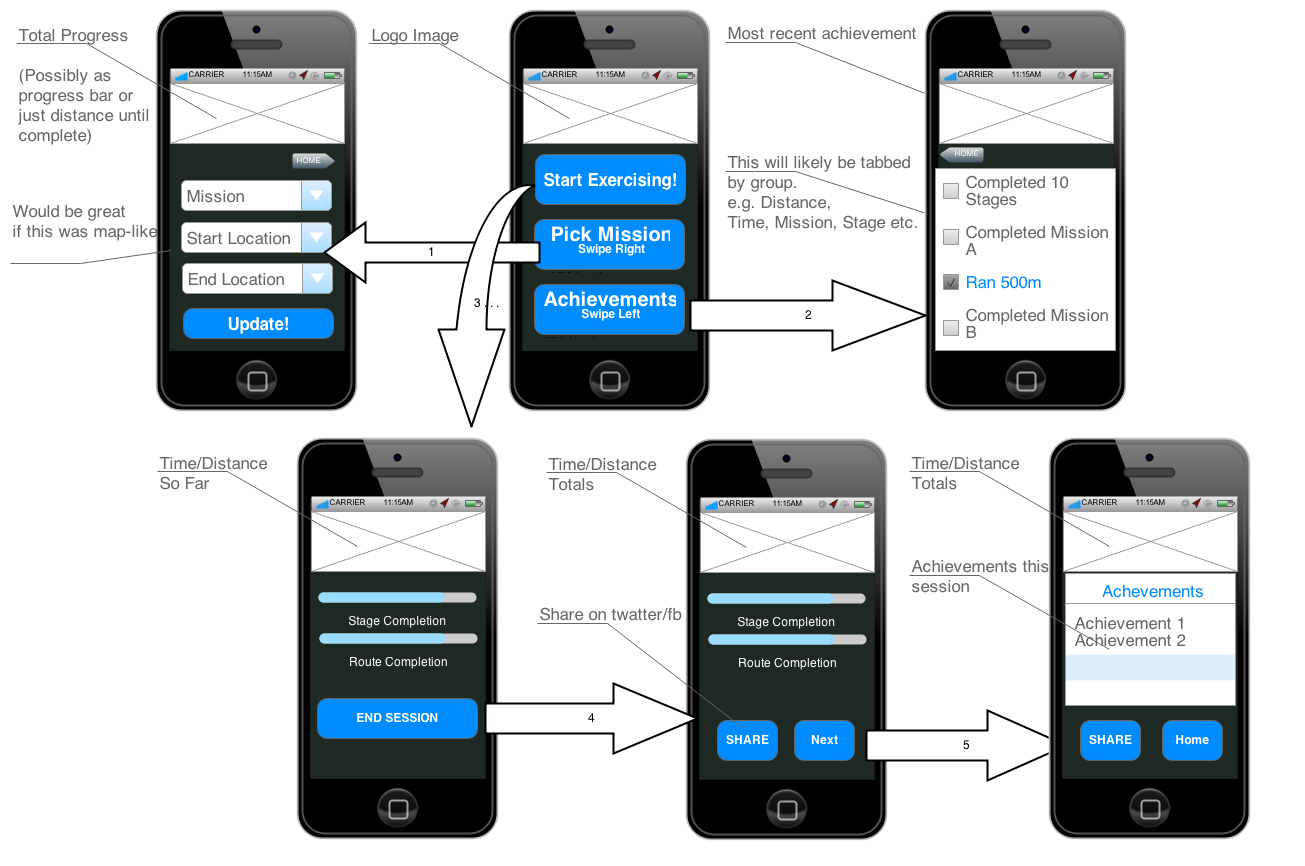
\includegraphics[width=\linewidth]{images/Wireframes.png}
  \caption{Wireframes, initial design}
  \label{wireframes_1}
\end{figure}
\begin{figure}[H]
  \centering
  \includegraphics[width=\linewidth]{images/wireframe_sketch.jpg}
  \caption{Inital sketch of wireframe ideas}
  \label{wireframes_2}
\end{figure}

\chapter{Installation Instructions}

The code can be checked out using git by executing the following:

git clone git@github.com:ryaanwells/urbanexplorer.git

Or by accessing the submitted files in $/local/lev4proj/2014/1002253w/Code$. Installation instructions are found at the following url:

\url{https://github.com/ryaanwells/urbanexplorer/blob/master/README.md}.


If any issues arise regarding installation of any part of the
system, do not hesitate to contact me at 

1002253w@student.gla.ac.uk


\bibliographystyle{plainnat}
\bibliography{wells-2013-urbanexplorer}
\end{document}
